\section{GT7: Aging Constants Are Run-Only: Freeze, Transfer, and the Scoreboard}
\label{sec:gt7}
%% Packet W-07. Ledger rows: GT7, NEG.gt7_transfer_failures.

\subsection{The protocol}

GT7 asks whether the numbers that characterize aging on East (Kovacs crossing time, peak time,
hump height, and three others) carry over to a different model without any fitting. The answer
was obtained the way a pre-registered experiment is \cite{nosek-et-al-2018,munafo-et-al-2017}: the readouts were fixed, the East reference
was computed, predictions for the target models were committed and hashed, and only then were the
targets run and scored by a script that had itself been frozen. Precisely:

\claimref{GT7}{4905b013624462549b9a4cdb18f51d0220f70be29976be461e5a8681978dcab8}
GT7's claim is a discipline plus its unedited outcome. The freeze-and-transfer protocol ran in
five stages, each frozen by sha256 content hash before the next began:

\begin{itemize}
  \item \textbf{F1, readouts freeze.} Six declared readouts (Kovacs $t_K$, $t_{\mathrm{peak}}$,
    hump height, memory-dimension profile, deficit-decay slope, cross-validation checks) frozen in
    a registry with content hash and freeze note.
  \item \textbf{F2, East reference.} The reference surface on East: 56 exact hump-surface cells
    at $N=10$, an $N=16$ Monte Carlo spot check, the closure-deficit ladder (Fig.~\ref{fig:deficit-decay}) whose declared secant slope is the
    frozen deficit-decay readout, and memory-dimension profiles. Run-only readouts; no functional form fitted anywhere.
  \item \textbf{F3, pre-registration.} 338 predictions committed before any target-family run:
    42 interval predictions, 2 order-relation predictions, and 294 cells explicitly declared
    \texttt{no\_prediction}. The predictions registry pins the frozen readouts hash, the East
    reference hash, and the hash of the scoring script itself.
  \item \textbf{F4, target runs.} FA and trap families run blind against the committed
    predictions.
  \item \textbf{F5, mechanical scoring.} The frozen scorer (hash-pinned at F3, verified
    unchanged) compares predictions to observations with no post-hoc widening or
    reinterpretation.
\end{itemize}

\begin{figure}[htbp]
  \centering
  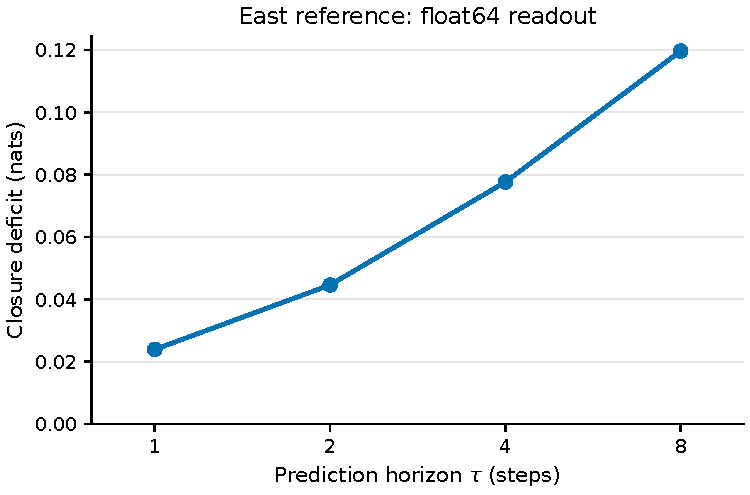
\includegraphics[width=0.7\linewidth]{figures/out/fig_gt7_deficit_decay.pdf}
  \caption{East-reference closure deficit (nats) across the declared $\tau$ ladder (run-only
    float64 readout; part of the frozen F2 reference). The frozen ``deficit-decay'' readout is the
    declared secant slope between two ladder points, not a fit; the deficit itself grows with
    horizon.}
  \label{fig:deficit-decay}
\end{figure}

\subsection{The scoreboard, unedited}

\claimref{NEG.gt7\_transfer\_failures}{37ac2b8f4bcb55cf1f2cf9f0518850a84039c3e51177d3000d0244b5ed6cc96e}
Of the 44 committed predictions, 22 were scored against observed target cells: \textbf{8 passed
and 14 failed}; the other 22 targeted cells that produced no observation. All 338 verdicts are
filed unedited (Fig.~\ref{fig:scoreboard}). The failure pattern is itself a filed, tested fact:

\begin{itemize}
  \item All 14 failures are FA-family interval predictions (5 $t_K$, 4 $t_{\mathrm{peak}}$,
    5 hump-height), and every one is \emph{one-sided high}: the observed FA value exceeds the
    predicted upper bound. FA humps are systematically later and larger than the East-anchored
    intervals allowed.
  \item Failures cluster at the deeper intermediate temperature: 12 of 14 failing cells have
    $\epsilon_{\mathrm{mid}} = 2/5$, where every scored cell failed. At
    $\epsilon_{\mathrm{mid}} = 1/2$, 7 of 9 scored interval cells passed (plus the passing
    order-relation prediction), and the two misses there are borderline (hump height $0.2033$
    against a bound of $0.2008$; $t_K$ of $5$ against $[1,3]$).
  \item All 22 unobserved cells are trap-family: the trap target's exact hump search returned
    \texttt{found = false} in all 56 surface cells, with the uniform miss reason ``does not start
    below equilibrium.'' This is the dynamical corollary of the $\epsilon$-invariance lemma of
    \S\ref{sec:models}: since the declared trap family's equilibrium does not move with
    $\epsilon$, a temperature jump never leaves it below its new equilibrium, and the Kovacs
    protocol cannot produce a hump there at all.
\end{itemize}

\begin{figure}[htbp]
  \centering
  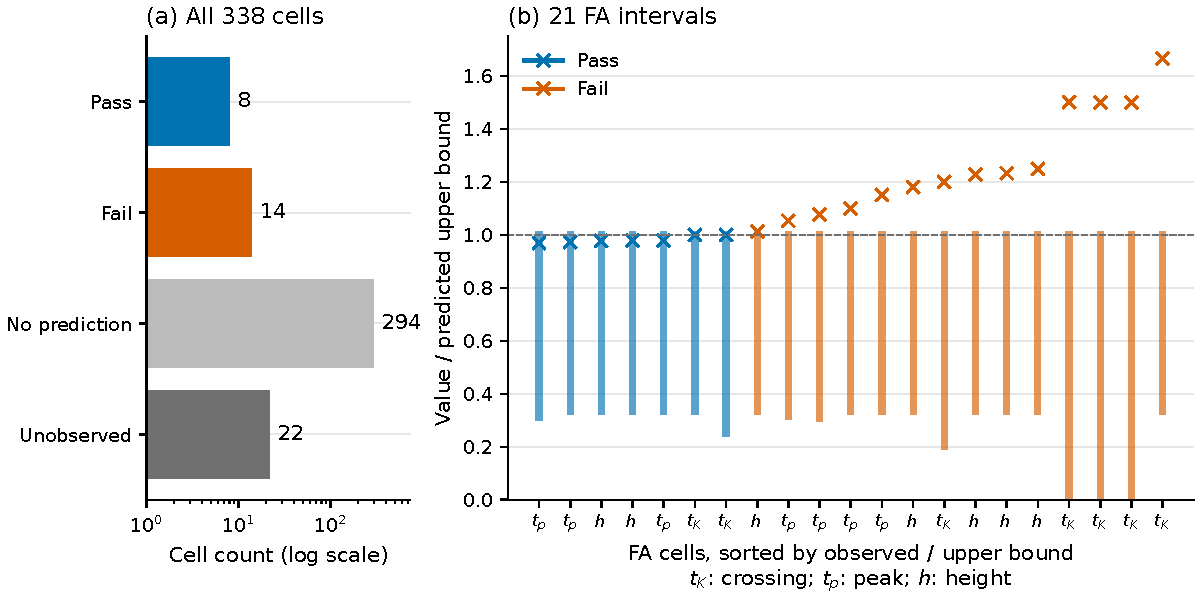
\includegraphics[width=\linewidth]{figures/out/fig_gt7_transfer_scoreboard.pdf}
  \caption{Left: verdict counts over all 338 cells (log scale). Right: the 21 scored FA interval cells
    (the 22nd scored FA prediction is the order relation, not plotted); each interval and its
    observed value are divided by the interval's upper bound, and cells are sorted by that ratio,
    so every failure lies above the dashed line at $1$.}
  \label{fig:scoreboard}
\end{figure}

\subsection{Reading the failures}

The failures are first-class results of the pre-registration protocol: it is designed to be
falsifiable, and it was. Three readings are compatible with the data, and the protocol forbids
choosing among them after the fact: (a) East-to-FA transfer of run-only constants degrades with
quench depth, in the direction of FA responding slower and larger; (b) the declared rule for
scaling East intervals to FA, rather than the readouts themselves, is what failed; (c) the trap
column is not a partial failure but a structural mismatch between the protocol and the declared
trap family, predicted in hindsight by the $\epsilon$-invariance lemma. Under any reading, the
run-only thesis stands as filed: the readouts are readouts of runs, frozen, transferred, and
scored, not fitted. (GT3's non-definability result concerns its own witness pair and the energy
lens; it is not extended here to the GT7 readouts, for which no such witness was constructed.) Score counts are not a fitted scaling law, and no post-hoc reinterpretation of failed
intervals is permitted or performed.
